
%(BEGIN_QUESTION)
% Copyright 2014, Tony R. Kuphaldt, released under the Creative Commons Attribution License (v 1.0)
% This means you may do almost anything with this work of mine, so long as you give me proper credit

Hvilken komponent, motstanden eller kondensatoren, vil få størst spenningsfall i denne kretsen?

$$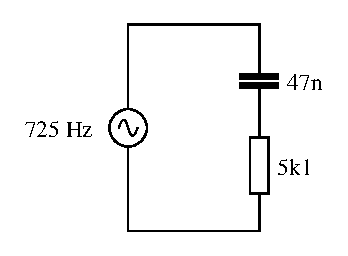
\includegraphics[width=15.5cm]{i01039x01.eps}$$

Beregn også total impedans ($Z_{total}$) i både rektangulær og polar form.

\underbar{file i01039}
%(END_QUESTION)





%(BEGIN_ANSWER)

Motstanden vil få størst spenningsfall.

\vskip 10pt

$Z_{total}$ (rektangulær) = 5100 $\Omega$ $-$ j4671 $\Omega$

\vskip 10pt

$Z_{total}$ (polar) = 6916 $\Omega$ $\angle$ $-42.5^{o}$

%(END_ANSWER)





%(BEGIN_NOTES)

Spør studentene hvilken metode som ga raskest beslutning om størst spenningsfall.

%INDEX% Electronics review: AC reactance and impedance

%(END_NOTES)

